\chapter{Организация консистентного хранилища данных}

\section*{Выбор хранилища данных}

\indent Система планирования производства, как и практически любая система получающая и обрабатывающая данные, нуждается в хранилище данных - базе данных.
Хранилище данных может быть разделено на две составляющие:
\begin{itemize}
	\item хранилище временных данных;
	\item хранилище постоянных данных.
\end{itemize}

\indent Под временными данными подразумеваются данные, которые получаются в процессе работы системы (например оперативные и объемно-календарные планы) и, при необходимости, могут быть рассчитаны заново, хоть и с некоторыми затратами (время, вычислительные мощности), при условии отсутствия хранилища данных.
В данной работе этот вид данных и хранилище для них не рассматривается.\\
\indent С другой стороны постоянные данные - данные, которые задаются пользователем (в данном случае организацией) и потеря которых в лучшем случае приведет к необходимости заново добавлять их в систему, а в худшем - приведет к утрате этих данных.
В любом случае потеря постоянных данных ведет к нарушениям в работе системы, что ведет к необходимости организации консистентного хранилища данных.\\
\indent Консистентность - требование к данным, получаемым из базы данных, которое заключается в том, что последние должны быть целостны и непротиворечивы.
Под целостностью данных подразумевается соответствие имеющейся в базе данных информации её внутренней логике, структуре и явно заданным правилам.
Любое правило, направленное на ограничение возможного состояния базы данных называют ограничением целостности.
Помимо целостных, данные должны также быть непротиворечивыми, что означает, что в базе данных нет логического противоречия, то есть некоторого утверждения и его отрицания.
Со стороны систем управления базами данных (совокупность программных и лингвистических средств общего или специального назначения, обеспечивающих управление созданием и использованием баз данных) свойство консистентности выполняется на уровне транзакций (одним из требований к которой и является консистентность): если одна из команд транзакции не прошла проверку ограничений целостности, то вся транзакция откатывается, то есть база данных возвращается в состояние, в котором была начата транзакция.\\
\indent Транзакция - группа последовательных операций с базой данных, которая представляет собой логическую единицу работы с данными.
Транзакция может либо быть целиком и успешно независимо от идущих параллельно транзакций и соблюдая все ограничения целостности, либо не быть выполненной вообще, что в таком случае не должно оказать на систему никакого влияния.\\
\indent В соответствии с требованиями описанными выше, можно сделать вывод о необходимости использования реляционной базы данных, одним из преимуществ которой является соответствие требованиям ACID (Atomicity, Consistency, Isolation, Durability - атомарность, консистентность, которая и интересует в первую очередь, изолированность, долговечность).

\section*{Структура базы данных}

\indent Из предыдущей главы видно, что в постоянной базе данных необходимо хранить информацию по которой будет производиться расчет объемно-календарного и оперативного планов.
Для этого необходимо хранить:

\begin{itemize}
	\item данные о заказах;
	\item данные о типах продукции;
	\item данные о продукции, которая относится к каждому заказу;
	\item данные о самой последовательности операций и самих операциях для каждого типа продукции;
	\item данные о каждой модели ресурсов;
	\item данные о связях между моделью ресурса и операциями.
\end{itemize}

\begin{figure}[ht]	
	\centering	
	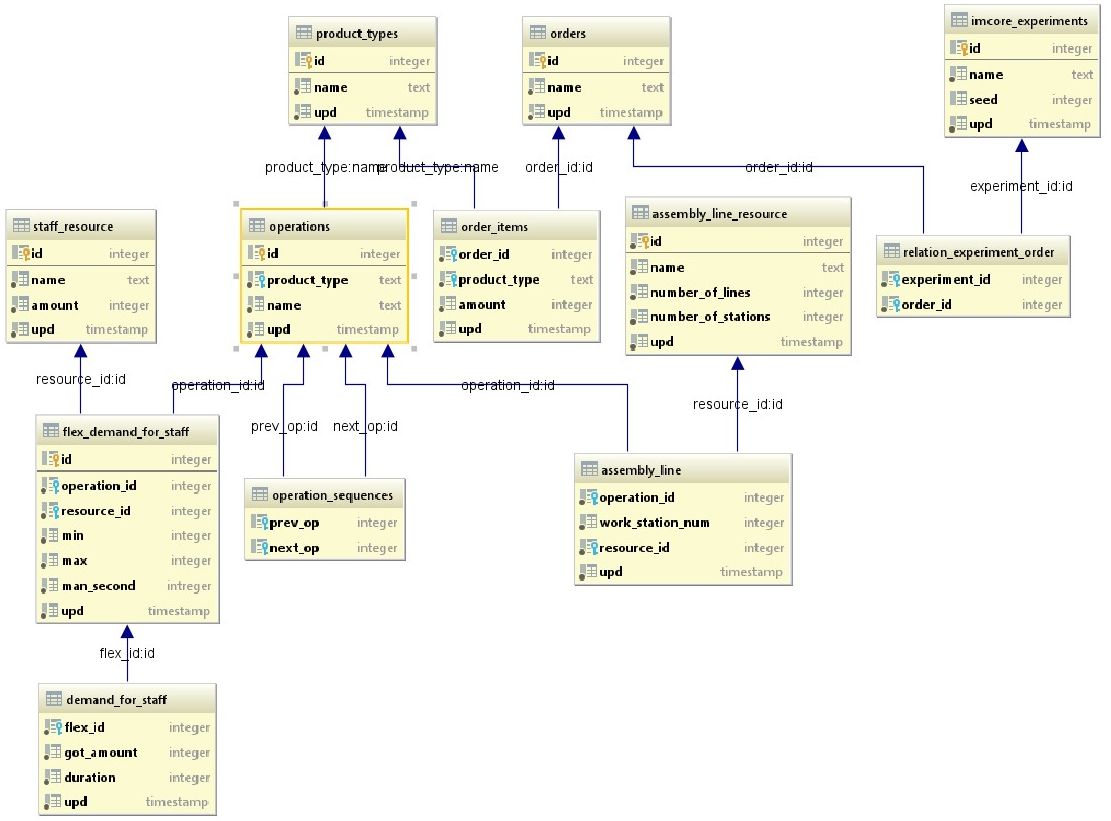
\includegraphics[width=\linewidth]{pics/databaseSchema.png}
	\caption{Схема базы данных}
	\label{fig:dbSchema}
\end{figure}

\indent Помимо этого, нужно учитывать, что кроме простого хранения данных, необходимо соблюдать 'версионность', ввиду того, что карта технологического процесса может меняться во времени, а значит и в базе данных, требуется следить за тем, чтобы в любой момент времени было возможно использовать любую из версий данной карты, иначе новый расчет оперативного плана (при условии, что другие данные остались неизменными) приведет к созданию новой версии плана, а, следовательно, предыдущую версию восстановить будет либо очень сложно, либо, в худшем случае - невозможно.\\
\indent Для достижения данной цели, в определенных таблицах было введено дополнительное поле - временная отметка обновления - 'upd'.
С помощью этой метки можно как получить последние данные из базы, просто максимизируя метку 'upd', так и получить данные на определенный момент времени ограничивая эту метку необходимым временем.

\section*{Обоснование/Доказательство}
\indent Теория реляционных баз данных оперирует понятиями отношения (relation), от которого и пошло само название теории и баз данных основанных на ней, атрибута, домена, кортежа.

\begin{figure}[ht]
	\centering
	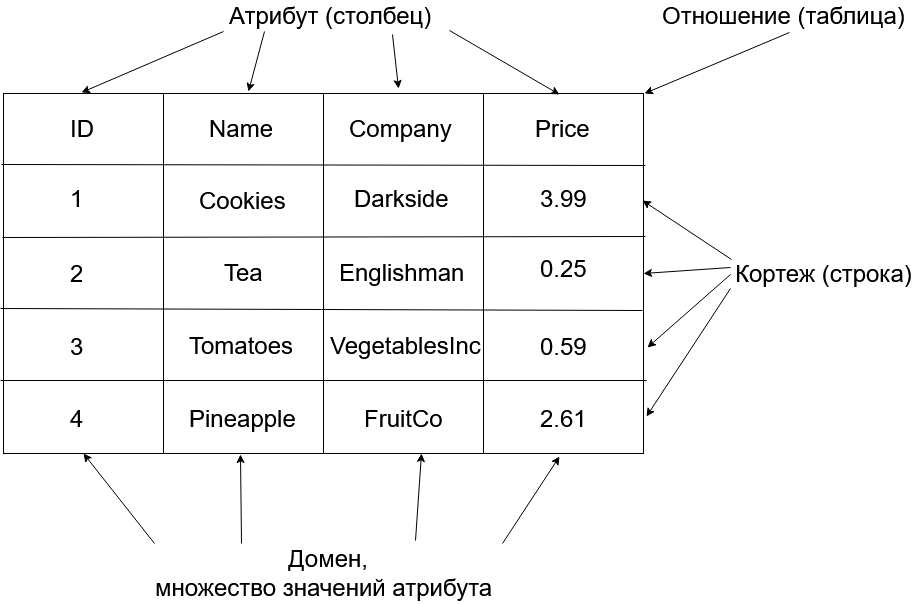
\includegraphics[width=\linewidth]{pics/databaseExample.png}
	\caption{Понятия реляционной базы данных}
	\label{fig:dbExample}
\end{figure}

\indent Атрибут - именованный столбец отношения.
В пределах одного атрибута все значения должны быть одного типа данных, то есть принадлежать одному домену.\\
\indent Домен - тип данных, множество всех допустимых значений атрибута.\\
\indent Кортеж - упорядоченный набор из N элементов, где N - это число атрибутов отношения.
По-другому можно сказать, что кортеж это строка или запись таблицы.\\
\indent Отношение - множество упорядоченных N-кортежей.
Другими словами отношение - это двумерная (плоская) таблица, состоящая из столбцов и строк - атрибутов и кортежей.(см. \ref{fig:dbExample})\\

\todo[inline]{математическое обоснование}
\todo[inline]{полностью переписать, исключить ACID}

\section{Теорема}
\begin{theorem}
	\label{th:th1}
	В любой момент времени можно восстановить необходимую версию карты технологического процесса, при условии того, что известно её имя и значение точки версионирования, которое не меньше заданного в базе данных для искомой карты и не больше и не равно следующей точки версионирования.
\end{theorem}

\begin{proof}[Доказательство]
	Используя метод доказательства от противного, предположим, что нельзя восстановить необходимую версию карты технологического процесса, при условии того, что известно её имя и значение точки версионирования, которое не меньше заданного в базе данных для искомой карты и не больше и не равно следующей точки версионирования из чего следует утверждение \ref{st:st1}.
	\begin{state}
		\label{st:st1}
		Нельзя создать такой запрос, который, для всех имён карт технологического процесса из домена 'name' отношения 'product\_types' и любой заданной точки версионирования построит нужную карту.
	\end{state}

	\begin{figure}[ht]
		\centering
		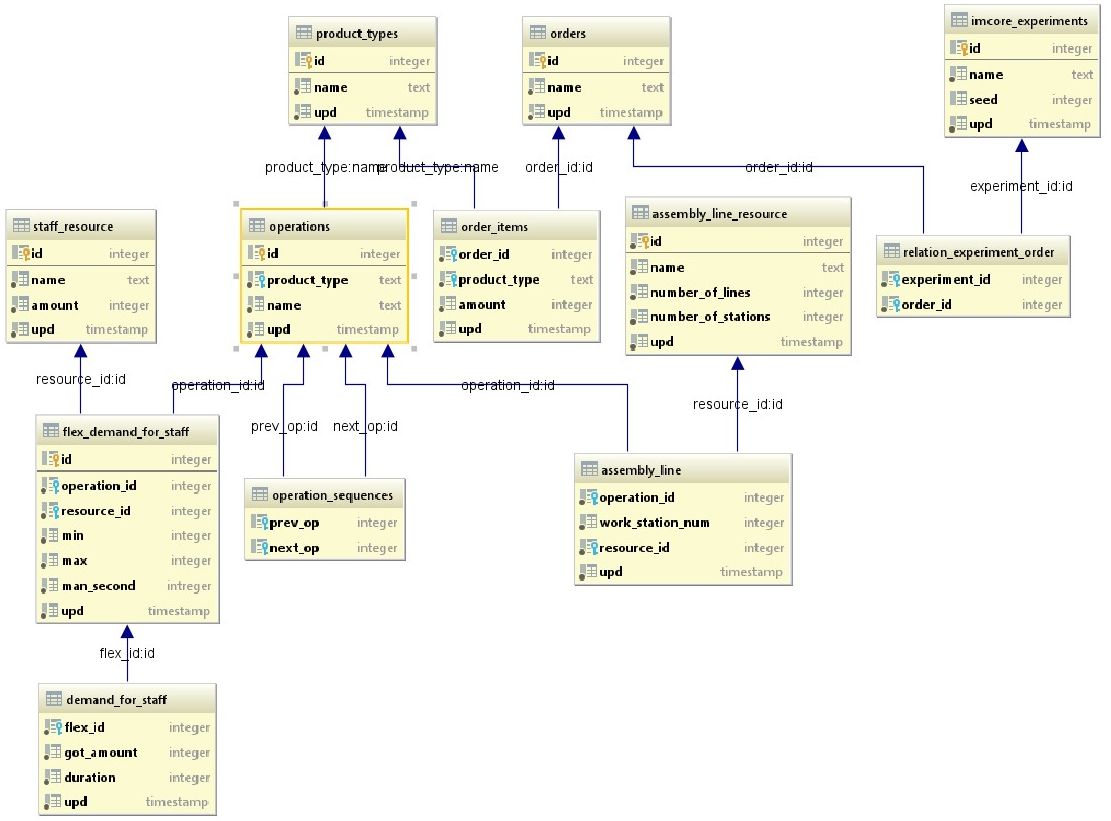
\includegraphics[width=\linewidth]{pics/databaseSchema.png}
		\caption{Схема базы данных}
		\label{fig:dbschema}
	\end{figure}

	\indent Используя схему БД, представленную на рисунке \ref{fig:dbschema}, постараемся доказать обратную теорему.\\
	\indent Введем сокращения названий отношений:

	\begin{itemize}
		\item $product\_types \Rightarrow pr$;
		\item $operations \Rightarrow ops$;
		\item $operation\_sequences \Rightarrow seq$.
	\end{itemize}

	\indent Предположим, есть переменная, принадлежащая домену 'name'\ отношения 'product\_types'\ $pr\_name \in pr.name$ и переменная $pr\_upd \in \mathbb{Z}$, заданные пользователем, тогда запишем запросы:
	\begin{equation}
		\label{eq:upd}
		pr\_upd' \leftarrow \pi_{pr.upd}(\sigma_{pr.name\ =\ pr\_name\ AND\ pr.upd\ \leq\ pr\_upd}\ pr)
	\end{equation}
	\begin{equation}
		\label{eq:ops}
		ops' \leftarrow \pi_{ops.id,\ pr.name,\ ops.upd}(pr \bowtie_{pr.name = ops.product\_type} ops)
	\end{equation}
	\begin{equation}
		\label{eq:seq}
		seq' \leftarrow \pi_{ops'.upd,\ ops'.name,\ seq.prev\_op,\ seq.next\_op}(ops' \bowtie_{ops'.id = seq.prev\_op} seq)
	\end{equation}
	\begin{equation}
		\label{eq:chart}
		chart \leftarrow \pi_{prev\_op,\ next\_op} (\sigma_{seq'.name\ =\ pr\_name\ AND\ seq'.upd\ =\ pr\_upd'\ } seq')
	\end{equation}

	\indent Проведем анализ полученных запросов:
	\begin{enumerate}
		\item[1)] в выражении \ref{eq:upd} производится извлечение значения ближайшей (и не большей чем заданная пользователем) точки версионирования;
		\item[2)] затем в выражении \ref{eq:ops} производится объединение отношений 'product\_types' и 'operations' по атрибуту имени карты технологического процесса, в результате получаем все операции всех карт технологического процесса всех точек версионирования;
		\item[3)] после этого в выражении \ref{eq:seq} объединяются отношение \ref{eq:ops} и 'operation\_sequences', что дает все последовательности операций для всех карт технологического процесса всех точек версионирования;
		\item[4)] и в \ref{eq:chart} производится выборка последовательностей из \ref{eq:seq} по имени карты процесса и полученной в выражении \ref{eq:upd} точки версионирования.
	\end{enumerate}

	\indent Так как карта технологического процесса записывается полностью и с одним значением точки версионирования для всех элементов, то мы получаем выборку карты, с заданным именем, которое существует в домене 'name' отношения 'product\_types' и с значением точки версионирования, которая существует в домене 'upd' того же отношения и, соответственно, является искомой картой.
	Создание такого запроса опровергает утверждение \ref{st:st1}, а следовательно доказывает теорему \ref{th:th1}.
\end{proof}